%%%%%%%%%%%%%%%%%%%%%%%%%%%%%%%%%%%%%%%%%%%%%%%%%%%%%%%%%%%%%%%%%%%%%%%%%%%%%
%%%
%%% File: thesis.tex, version 1.9, May 2016
%%%
%%% =============================================
%%% This file contains a template that can be used with the package
%%% cs.sty and LaTeX2e to produce a thesis that meets the requirements
%%% of the Computer Science Department from the Technical University of Cluj-Napoca
%%%%%%%%%%%%%%%%%%%%%%%%%%%%%%%%%%%%%%%%%%%%%%%%%%%%%%%%%%%%%%%%%%%%%%%%%%%%%

\documentclass[12pt,a4paper,twoside]{report}         
\usepackage{cs}              
\usepackage{times}
\usepackage{graphicx}
\usepackage{latexsym}
\usepackage{amsmath,amsbsy}
\usepackage{amssymb}
\usepackage[matrix,arrow]{xy}
\usepackage[T1]{fontenc}
\usepackage{ae,aecompl}
\usepackage{romanian} %definitii pentru diacritice; 
\usepackage{amstext}
\usepackage{graphics}
\usepackage[T1]{fontenc}
\usepackage{ae,aecompl}
%\usepackage{algorithm}
%\usepackage{algorithmic}
\usepackage{color}
\usepackage{color}
\usepackage{listings}
\usepackage{verbatim}
\usepackage{subcaption}

\usepackage{algorithm2e}


% \mastersthesis
\diplomathesis
% \leftchapter
\centerchapter
% \rightchapter
\singlespace
% \oneandhalfspace
% \doublespace

\renewcommand{\thesisauthor}{Nicoleta COROCEA}    %% Your name.
\renewcommand{\thesismonth}{Iunie}     %% Your month of graduation.
\renewcommand{\thesisyear}{2019}      %% Your year of graduation.
\renewcommand{\thesistitle}{EXPLAINABLE MACHINE LEARNING USING ONTOLOGIES } % Title
\renewcommand{\thesissupervisor}{Assoc.Prof.Dr.Eng. Adrian GROZA}
\newcommand{\department}{FACULTATEA DE AUTOMATIC'A 'SI CALCULATOARE\\
DEPARTAMENTUL CALCULATOARE}
\newcommand{\thesis}{LUCRARE DE LICEN'T'A}
\newcommand{\uline}[1]{\rule[0pt]{#1}{0.4pt}}
%\renewcommand{\thesisdedication}{P'arin'tilor mei}
\newcommand{\utcnlogo}{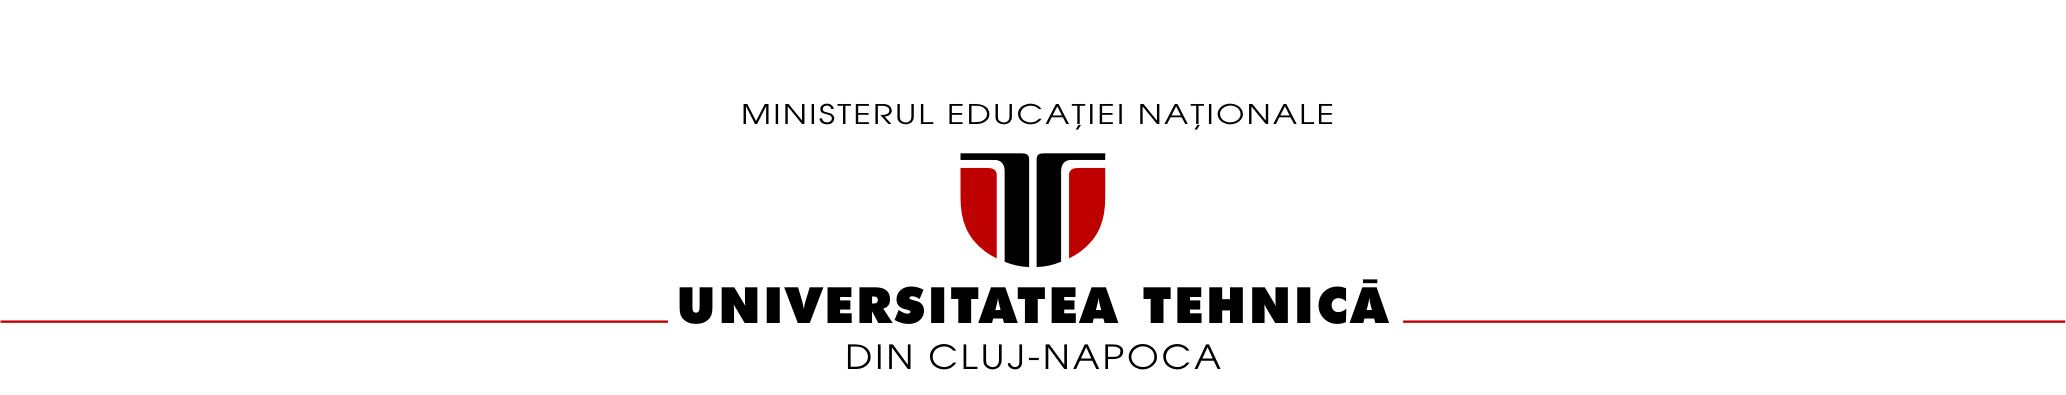
\includegraphics[width=15cm]{img/utcn.jpg}}
\newtheorem{example}{Exemplu}
\begin{document}


\section{Cerin'tele sistemului}

\subsection{Cerin'te func'tionale}

\begin{itemize}
    \item {\it Translatarea limbajului natural 'in SPARQL} - Sistemul trebuie s'a pun'a la dispozi'tie un mecanism de translatare a 'intreb'arilor din limbaj natural 'in limbaj de interogare SPARQL, precum 'si o modalitate de editare ulterioar'a a interog'arilor.
    \item {\it Interogarea\ ontologiei} -  Sistemul trebuie s'a permit'a interogarea ontologiei utiliz\ia nd limbajul de interogare SPARQL destinat ontologiilor 'si s'a ofere r'aspunsuri pe baza resurselor conceptualizate 'in baza de cuno'stin'te, utiliz\ia nd libr'aria Pellet 'si libr'aria RDFLib.
    \item {\it Permite\ vizualizarea\ elementelor\ ontologiei} - Sistemul trebuie s'a ofere capabilitatea de a expune, prin intermediul interfe'tei utilizator, a tuturor elementelor din care este constituit'a ontologia.
\end{itemize}
\subsection{Cerin'te nonfunc'tionale}
\begin{itemize}
    \item {\it Utilizabilitate} - Proiectarea sistemului 'si a interfe'tei utilizator se va face urm'arind simplitatea de utilizare. Clien'tii novici pot 'incepe utilizarea cu pu'tin instructaj asupra utiliz'arii aplica'tiei.
    \item {\it Toleran'ta\ la\ e'sec} - Sistemul este construit 'in a'sa fel 'inc\ia t, 'in cazul in care acesta e'sueaz'a 'in interpretarea intreb'arii sau pentru g'asirea unui r'aspuns, utilizatorul va fi rugat s'a repete 'intrebarea sub o alta forma sau s'a verifice interogarea.
    \item {\it Securitate} - Datele ontologiei pot fi vizualizate, fiind publice utilizatorilor, dar nu se va permite realizarea interog'arilor care pot modifica  sau altera starea acestora.
    \item {\it Explicativ} - Realizarea sistemului va 'tine cont de transparen'ta de realizare a opera'tiilor, c'at si de dreptul utilizatorului de a fi implicat 'in procesul de decizie.
\end{itemize}


\end{document}